\documentclass{minimal}
\usepackage[T1]{fontenc}
\usepackage{newtxtext}
\usepackage{newtxmath}
\renewcommand{\sffamily}{\rmfamily}
\usepackage{tikz}
\usetikzlibrary{arrows.meta,calc,positioning}
\usepackage{xcolor}

\definecolor{ink}{HTML}{1F2933}
\definecolor{muted}{HTML}{59636E}
\definecolor{paper}{HTML}{FFFFFF}
\definecolor{panel}{HTML}{F7F9FA}
\definecolor{blue}{HTML}{315F80}
\definecolor{bluefill}{HTML}{EAF1F5}
\definecolor{green}{HTML}{2F6B58}
\definecolor{greenfill}{HTML}{E7F2ED}
\definecolor{purple}{HTML}{62578A}
\definecolor{purplefill}{HTML}{EEEAF5}
\definecolor{orange}{HTML}{A85B1A}
\definecolor{orangefill}{HTML}{FBF0E4}
\definecolor{grayfill}{HTML}{F0F2F3}

\pdfpagewidth=1000pt
\pdfpageheight=430pt
\setlength{\paperwidth}{1000pt}
\setlength{\paperheight}{430pt}
\setlength{\textwidth}{1000pt}
\setlength{\textheight}{430pt}
\setlength{\oddsidemargin}{-72pt}
\setlength{\topmargin}{-72pt}
\setlength{\headheight}{0pt}
\setlength{\headsep}{0pt}
\setlength{\footskip}{0pt}
\setlength{\parindent}{0pt}
\pagestyle{empty}

\begin{document}
\begin{tikzpicture}[
  x=1pt,y=1pt,
  font=\sffamily,
  line cap=round,
  line join=round,
  inference/.style={-{Latex[length=9pt,width=6pt]},draw=ink,line width=2.2pt},
  supervision/.style={-{Latex[length=8pt,width=5pt]},draw=orange,
                      densely dashed,line width=2.0pt},
  intervention/.style={-{Latex[length=7pt,width=5pt]},draw=muted,
                       densely dotted,line width=1.8pt},
  module/.style={rounded corners=8pt,draw=ink,line width=1.6pt,
                 fill=paper,align=center,minimum height=50pt},
  input/.style={module,fill=bluefill},
  state/.style={module,fill=greenfill},
  transition/.style={module,fill=purplefill},
  closure/.style={module,fill=orangefill},
  condition/.style={rounded corners=9pt,draw=purple,line width=1.3pt,
                    fill=paper,minimum height=25pt,align=center},
  trainnode/.style={rounded corners=7pt,draw=orange,line width=1.4pt,
                    fill=paper,align=center,minimum height=34pt},
  probe/.style={rounded corners=7pt,draw=muted,line width=1.25pt,
                fill=paper,align=center,minimum height=36pt},
  optional/.style={probe,densely dashed,fill=grayfill,draw=muted!80}
]
\useasboundingbox (0,0) rectangle (1000,430);
\fill[paper] (0,0) rectangle (1000,430);

% Compact heading and line-style key.
\node[anchor=west,text=ink,font=\sffamily\bfseries\fontsize{20}{23}\selectfont]
  at (22,412) {TerraState forecast closure};
\draw[inference] (405,412) -- (446,412);
\node[anchor=west,text=muted,font=\sffamily\fontsize{19}{22}\selectfont]
  at (454,412) {inference};
\draw[supervision] (558,412) -- (599,412);
\node[anchor=west,text=muted,font=\sffamily\fontsize{19}{22}\selectfont]
  at (607,412) {training only};
\draw[intervention] (743,412) -- (784,412);
\node[anchor=west,text=muted,font=\sffamily\fontsize{19}{22}\selectfont]
  at (792,412) {post-training};

% Inference is the dominant visual layer.
\draw[rounded corners=12pt,fill=panel,draw=ink!20,line width=1.1pt]
  (18,199) rectangle (982,393);
\node[anchor=west,text=ink,font=\sffamily\bfseries\fontsize{20}{23}\selectfont]
  at (31,379) {History-only state inference};
\node[anchor=west,text=purple,font=\sffamily\bfseries\fontsize{20}{23}\selectfont]
  at (492,379) {Weather-driven state transition};
\node[anchor=west,text=orange,font=\sffamily\bfseries\fontsize{20}{23}\selectfont]
  at (824,379) {Forecast closure};

\node[input,minimum width=140pt,minimum height=72pt] (history) at (84,280) {};
\draw[draw=blue,line width=1.1pt,fill=paper] (49,289) rectangle (73,308);
\draw[draw=blue,line width=1.1pt,fill=bluefill] (60,292) rectangle (84,311);
\draw[draw=blue,line width=1.1pt,fill=greenfill] (71,295) rectangle (95,314);
\draw[draw=muted,line width=1.1pt] (74,299) -- (92,299);
\draw[draw=muted,line width=1.1pt] (74,304) -- (92,304);
\draw[draw=muted,line width=1.1pt] (78,296) -- (78,312);
\draw[draw=muted,line width=1.1pt] (85,296) -- (85,312);
\node[text=ink,align=center,font=\sffamily\bfseries\fontsize{19}{22}\selectfont]
  at (84,266) {cloud-masked\\EO history};
\node[condition,minimum width=142pt,
      font=\sffamily\bfseries\fontsize{19}{22}\selectfont]
  (contextaux) at (171,341) {past meteorology\\+ static $g$};
\node[input,minimum width=145pt,minimum height=62pt,text width=136pt,
      font=\sffamily\bfseries\fontsize{20}{23}\selectfont]
  (q) at (247,280) {history-only $q_\theta$\\[-1pt]
                    \normalfont\fontsize{19}{22}\selectfont context encoder};
\node[input,minimum width=72pt,font=\sffamily\bfseries\fontsize{21}{24}\selectfont]
  (proj) at (385,280) {$P_\rho$};
\node[state,minimum width=84pt,font=\sffamily\bfseries\fontsize{19}{22}\selectfont]
  (zt) at (475,280) {$z_t$};
\node[transition,minimum width=112pt,minimum height=62pt,
      font=\sffamily\bfseries\fontsize{21}{24}\selectfont]
  (trans) at (607,280) {shared $T_\psi$};
\node[state,minimum width=90pt,font=\sffamily\bfseries\fontsize{19}{22}\selectfont]
  (zh) at (710,280) {$z_{t+h}$};
\node[closure,minimum width=80pt,text width=72pt,
      font=\sffamily\bfseries\fontsize{20}{23}\selectfont]
  (odecode) at (805,280) {closure\\$O_\omega$};
\node[circle,draw=ink,line width=1.8pt,fill=paper,minimum size=37pt,
      font=\sffamily\bfseries\fontsize{23}{26}\selectfont]
  (plus) at (870,280) {$+$};
\node[closure,minimum width=91pt,minimum height=72pt,text width=82pt]
  (pred) at (944,280) {};
\draw[draw=orange,line width=1.1pt,fill=paper] (923,293) rectangle (965,309);
\draw[draw=orange!65,line width=1.1pt] (937,293) -- (937,309);
\draw[draw=orange!65,line width=1.1pt] (951,293) -- (951,309);
\draw[draw=orange!65,line width=1.1pt] (923,301) -- (965,301);
\node[text=ink,font=\sffamily\bfseries\fontsize{19}{22}\selectfont]
  at (944,276) {forecast};
\node[text=ink,font=\sffamily\fontsize{19}{22}\selectfont]
  at (944,255) {$\widehat y_{t+h}$};

\draw[inference] (history.east) -- (q.west);
\draw[inference,line width=1.5pt] (contextaux.south) -- ($(q.north)+(0,0)$);
\draw[inference] (q.east) -- (proj.west);
\draw[inference] (proj.east) -- (zt.west);
\draw[inference] (zt.east) -- (trans.west);
\draw[inference] (trans.east) -- (zh.west);
\draw[inference] (zh.east) -- (odecode.west);
\draw[inference] (odecode.east) -- node[above,text=muted,
  font=\sffamily\fontsize{19}{22}\selectfont] {$r_h$} (plus.west);
\draw[inference] (plus.east) -- (pred.west);

\node[condition,minimum width=116pt,
      font=\sffamily\bfseries\fontsize{19}{22}\selectfont]
  (weather) at (541,341) {full24 future\\weather};
\node[condition,minimum width=76pt,
      font=\sffamily\bfseries\fontsize{19}{22}\selectfont]
  (transgeo) at (660,341) {static $g$};
\node[condition,minimum width=82pt,
      font=\sffamily\bfseries\fontsize{19}{22}\selectfont]
  (horizon) at (752,341) {horizon $h$};
\draw[inference,line width=1.5pt] (weather.south) -- ($(trans.north)+(-31pt,0)$);
\draw[inference,line width=1.5pt] (transgeo.south) -- (trans.north);
\draw[inference,line width=1.5pt] (horizon.south) -- ($(trans.north)+(31pt,0)$);

% The context prior is emitted before future weather is introduced.
\node[input,minimum width=157pt,font=\sffamily\bfseries\fontsize{19}{22}\selectfont]
  (prior) at (417,218) {context-only prior $b_h$};
\draw[inference] ($(q.south)+(0,0)$) |- (prior.west);
\draw[inference] (prior.east) -- ++(247pt,0) |- (plus.south);

% Training signals are explicitly separated from inference.
\draw[rounded corners=11pt,fill=orangefill,draw=orange!55,line width=1.2pt]
  (18,80) rectangle (982,187);
\node[anchor=west,text=orange,font=\sffamily\bfseries\fontsize{20}{23}\selectfont]
  at (31,174) {Training only:\quad
  $\mathcal L=\mathcal L_{\mathrm{GT}}+0.5\mathcal L_{\mathrm{KD}}
  +\lambda_s\mathcal L_{\mathrm{future\mbox{-}state}}$};

\node[trainnode,minimum width=250pt,text width=236pt,minimum height=42pt,
      font=\sffamily\fontsize{19}{22}\selectfont]
  (gtcard) at (153,125)
  {\textbf{Forecast target}\\[-1pt]
   $\mathcal L_{\mathrm{GT}}(\widehat y_{t+h},y_{t+h})$};
\node[trainnode,minimum width=270pt,text width=256pt,minimum height=42pt,
      font=\sffamily\fontsize{19}{22}\selectfont]
  (kdcard) at (438,125)
  {\textbf{Frozen full-weather teacher}\\[-1pt]
   $\mathcal L_{\mathrm{KD}}(\widehat y_{t+h},
   \widehat y^{\mathrm{teach}}_{t+h})$};
\node[trainnode,minimum width=363pt,text width=349pt,minimum height=50pt,
  font=\sffamily\fontsize{19}{22}\selectfont]
  (statecard) at (791,125)
  {\textbf{Future-state anchor ($h=20$ only)}\\[-1pt]
   observed future EO $\longrightarrow$ frozen $q_\theta+P_\rho$ /
   cached $z^\star_{t+20}$};

\draw[supervision] (zh.south) -- (710,187);
\draw[supervision] (pred.south) -- (944,187);

% Compact verification strip: evidence for the same model, not a co-equal benchmark.
\draw[rounded corners=9pt,fill=grayfill,draw=muted!55,line width=1.1pt]
  (18,9) rectangle (982,74);
\node[anchor=west,align=left,text width=148pt,text=ink,
      font=\sffamily\bfseries\fontsize{19}{22}\selectfont]
  at (30,41) {Same checkpoint\\post-training tests};
\draw[intervention] (187,41) -- (213,41);

\node[probe,minimum width=132pt,font=\sffamily\fontsize{19}{22}\selectfont]
  (q1) at (286,41) {\textbf{\color{blue}Q1 Forecast}\\frozen checkpoint};
\node[probe,minimum width=186pt,font=\sffamily\fontsize{19}{22}\selectfont]
  (q2) at (455,41) {\textbf{\color{blue}Q2 Load-bearing}\\full \quad cut \quad $T\!\to\!I$};
\node[probe,minimum width=189pt,font=\sffamily\fontsize{19}{22}\selectfont]
  (q3) at (657,41) {\textbf{\color{green}Q3 Driver response}\\matched \quad mean \quad donor};
\node[optional,minimum width=199pt,font=\sffamily\fontsize{19}{22}\selectfont]
  (q4) at (872,41) {\textbf{\color{muted}Q4 Optional}\\direct $\cdot$ composed $\cdot$ guards};

\end{tikzpicture}
\end{document}
